\documentclass{beamer}
%%%%%%%%%%%%%%%%%%%%%%%%%%%%%%%%%%%%%%%%%%%%%%%%%%%%%%%%%%%%%%%%%%%%%%%%%%%%%%%%%%%%%%%%%%%%%%%%%%
\setbeamertemplate{navigation symbols}{}
\usepackage{beamerthemeshadow}
\usefonttheme{serif}
%%%%%%%%%%%%%%%%%%%%%%%%%%%%%%%%%%%%%%%%%%%%%%%%%%%%%%%%%%%%%%%%%%%%%%%%%%%%%%%%%%%%%%%%%%%%%%%%%%
\usepackage{graphicx}
\graphicspath{ {res/} }
%%%%%%%%%%%%%%%%%%%%%%%%%%%%%%%%%%%%%%%%%%%%%%%%%%%%%%%%%%%%%%%%%%%%%%%%%%%%%%%%%%%%%%%%%%%%%%%%%%
\usepackage{polyglossia}
\setdefaultlanguage{armenian}
\setotherlanguages{english}
\usepackage{fontspec}
\newfontfamily\armenianfont{DejaVu Sans}
%%%%%%%%%%%%%%%%%%%%%%%%%%%%%%%%%%%%%%%%%%%%%%%%%%%%%%%%%%%%%%%%%%%%%%%%%%%%%%%%%%%%%%%%%%%%%%%%%%
\usepackage{minted}
\setminted[cpp]{fontsize=\footnotesize}
\setmonofont{Consolas}
%%%%%%%%%%%%%%%%%%%%%%%%%%%%%%%%%%%%%%%%%%%%%%%%%%%%%%%%%%%%%%%%%%%%%%%%%%%%%%%%%%%%%%%%%%%%%%%%%%
\usepackage{xltxtra}
\usepackage{hyperref}
%%%%%%%%%%%%%%%%%%%%%%%%%%%%%%%%%%%%%%%%%%%%%%%%%%%%%%%%%%%%%%%%%%%%%%%%%%%%%%%%%%%%%%%%%%%%%%%%%%
\usetheme{Luebeck}
\usecolortheme{crane}
%%%%%%%%%%%%%%%%%%%%%%%%%%%%%%%%%%%%%%%%%%%%%%%%%%%%%%%%%%%%%%%%%%%%%%%%%%%%%%%%%%%%%%%%%%%%%%%%%%
\definecolor{HTDark}{rgb}{0.04706, 0.13725, 0.26667} % primary color
\definecolor{HTLight}{rgb}{0.3686, 0.5255, 0.6235}   % secondary color
\setbeamercolor{palette primary}{bg=HTDark,fg=white}
\setbeamercolor{palette secondary}{bg=HTDark,fg=white}
\setbeamercolor{palette tertiary}{bg=HTDark,fg=white}
\setbeamercolor{palette quaternary}{bg=HTDark,fg=white}
\setbeamercolor{structure}{fg=HTDark} % itemize, enumerate, etc
\setbeamercolor{section in toc}{fg=HTDark} % TOC sections
\setbeamercolor{block title}{fg=white,bg=HTDark}
\setbeamercolor{block body}{fg=white, bg=HTLight}
\setbeamercolor{subsection in head/foot}{bg=HTLight,fg=white}
%%%%%%%%%%%%%%%%%%%%%%%%%%%%%%%%%%%%%%%%%%%%%%%%%%%%%%%%%%%%%%%%%%%%%%%%%%%%%%%%%%%%%%%%%%%%%%%%%%

\begin{document}

\title[FactoryMethod]{Նախագծման Ձևանմուշներ։ FactoryMethod}
\author[Հրաչյա Թանդիլյան\copyright]{Հրաչյա Թանդիլյան}
\date{2020}

%-------------------------------------------------------------------------------------------------
\begin{frame}
\titlepage
\end{frame}
%-------------------------------------------------------------------------------------------------

\section{Նպատակը}
%-------------------------------------------------------------------------------------------------
\begin{frame}\frametitle{FactoryMethod}
\begin{block}{Նպատակը}
    Ինտերֆեյս է սահմանում օբյեկտ ստեղծելու համար,
    սակայն ենթադասերին թույլ է տալիս որոշել ստեղծվելիք օբյեկտի տիպը: \\
    \vspace{0.5cm}
    Այսինքն այն թույլ է տալիս զիջել օբյեկտի ստեղծումը ենթադասերին:
\end{block}
\vfill
Նաև հայտնի է որպես
\begin{itemize}
    \item Virtual Constructor
\end{itemize}
\end{frame}
%-------------------------------------------------------------------------------------------------

\subsection{Մոտիվացիան}
%-------------------------------------------------------------------------------------------------
\begin{frame}\frametitle{Մոտիվացիան}
\begin{center}
    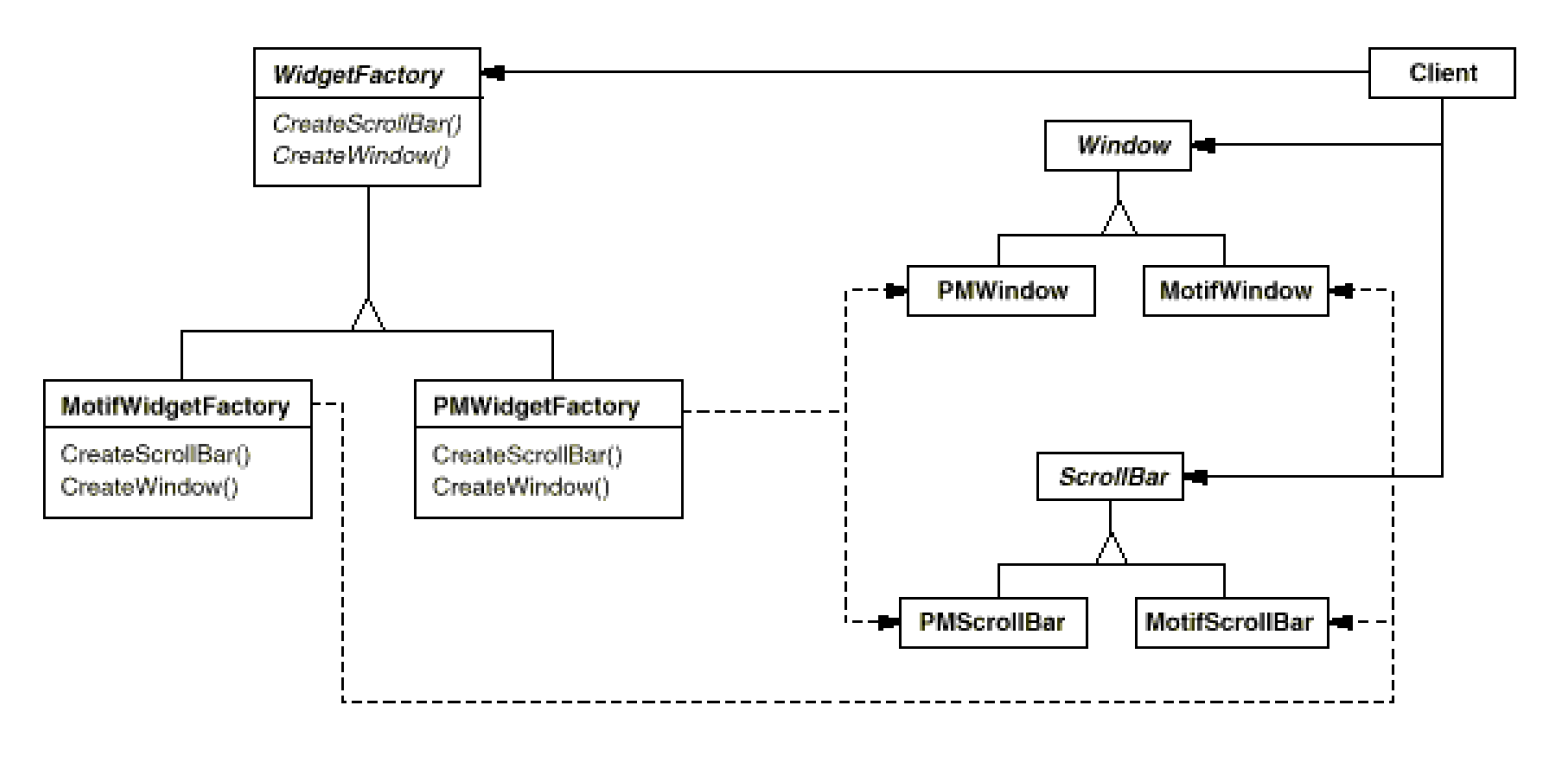
\includegraphics[scale=0.28]{motivation.png}
\end{center}
\end{frame}
%-------------------------------------------------------------------------------------------------

\subsection{Կիրառելիությունը}
%-------------------------------------------------------------------------------------------------
\begin{frame}\frametitle{Կիրառելիությունը}
Այս Ն.Ձ. պետք է օգտագործել երբ.
\vfill
\begin{enumerate}
    \item Դասը չի կարող կանխատեսել ստեղծվելիք օբյեկտի տիպը: \pause \vfill
    \item Անհրաժեշտ է, որ դասի ենթադասերը որոշեն ստեղծվելիք օբյեկտի տիպը: \pause \vfill
    \item Դասը փոխանցում է պատասխանատվությունը մի քանի օգնական դասերի և
     անհրաժեշտ է լոկալիզացնել, թե որ օգնական դասին է փոխանցվել պատասխանատվությունը:
\end{enumerate}
\end{frame}
%-------------------------------------------------------------------------------------------------

\section{Կառուցվածքը}
%-------------------------------------------------------------------------------------------------
\begin{frame}\frametitle{Կառուցվածքը}
\begin{center}
    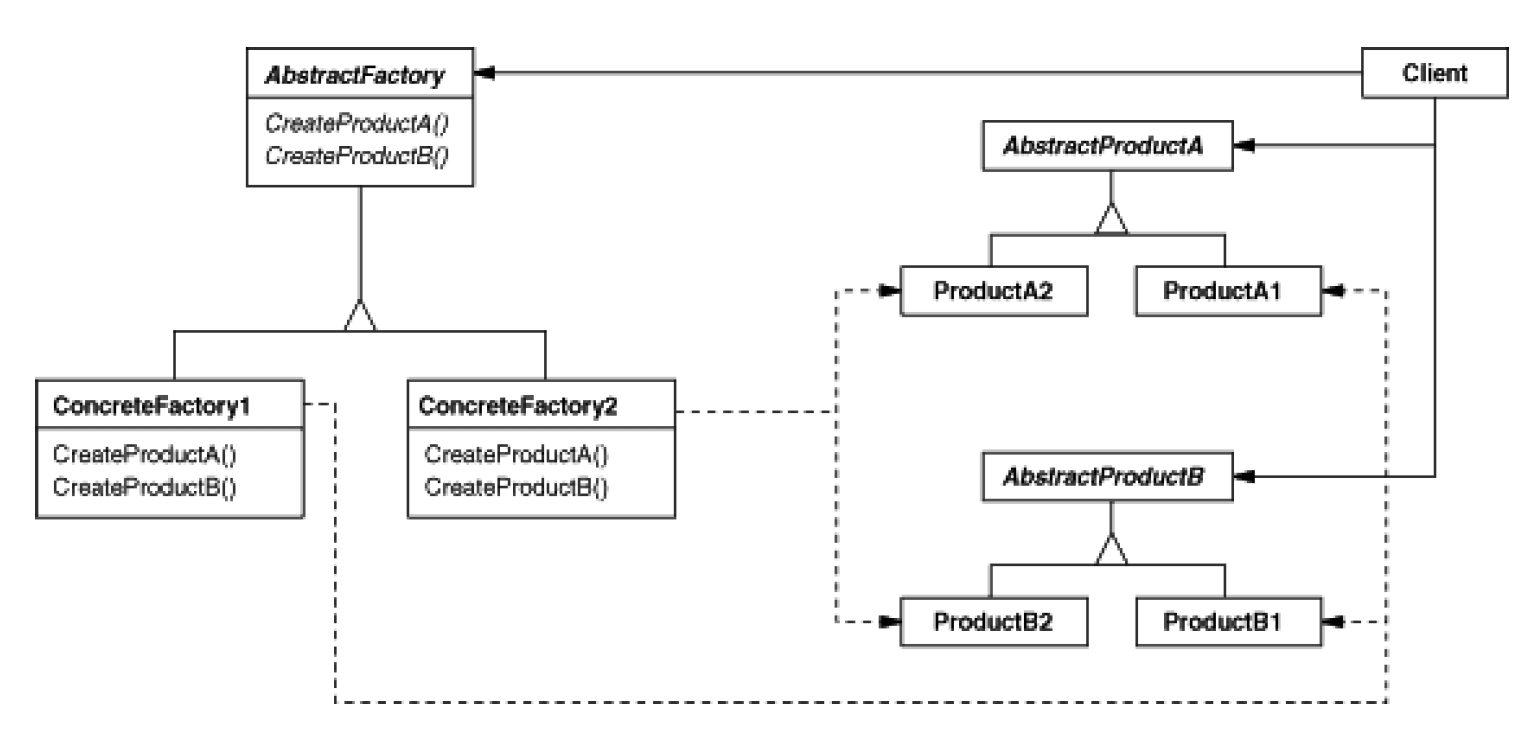
\includegraphics[scale=0.3]{structure.png}
\end{center}
\end{frame}
%-------------------------------------------------------------------------------------------------

\subsection{Հետևանքները}
%-------------------------------------------------------------------------------------------------
\begin{frame}\frametitle{Հետևանքները}
Այս Ն.Ձ. ունի հետևյալ առավելություններն ու թերությունները.
\vfill
\begin{enumerate}
    \item Վերացնում է կիրառությանը հատուկ դասերին հղվելու անհրաժեշտությունը կոդում: \pause \vfill
    \item Առաջացնում է հավելյալ ժառանգության վտանգ: \pause \vfill
    \item Ապահովում է ճկունություն ենթադասերի համար: \pause \vfill
    \item Կապ է ստեղծում դասերի զուգահեռ հիերարխիաների միջև:
\end{enumerate}
\end{frame}
%-------------------------------------------------------------------------------------------------

\section{Իրականացումը}
%-------------------------------------------------------------------------------------------------
\begin{frame}\frametitle{Իրականացումը}
\begin{enumerate}
    \item Երկու հիմնական տարբերակներ: \vspace{0.5cm}
    \item Պարամետրիզացված Factory Method: \vfill
\end{enumerate}
\end{frame}
%-------------------------------------------------------------------------------------------------

%-------------------------------------------------------------------------------------------------
\begin{frame}[fragile]\frametitle{Պարամետրիզացված FactoryMethod}
\begin{english}
\begin{minted}{cpp}
class Creator {
    public:
    virtual Product* Create(ProductId);
};

Product* Creator::Create(ProductId id) {

    if (id == MINE) return new MyProduct;

    if (id == YOURS) return new YourProduct;

    // repeat for remaining products
    return 0;
}
\end{minted}
\end{english}
\end{frame}
%-------------------------------------------------------------------------------------------------

%-------------------------------------------------------------------------------------------------
\begin{frame}[fragile]\frametitle{Պարամետրիզացված FactoryMethod}
\begin{english}
\begin{minted}{cpp}
Product* MyCreator::Create(ProductId id) {

    if (id == YOURS) return new MyProduct;

    if (id == MINE) return new YourProduct;

    // switched YOURS and MINE

    if (id == THEIRS) return new TheirProduct;

    return Creator::Create(id); // called if all others fail
}
\end{minted}
\end{english}
\end{frame}
%-------------------------------------------------------------------------------------------------

%-------------------------------------------------------------------------------------------------
\begin{frame}\frametitle{Իրականացումը}
\begin{enumerate}
    \item Երկու հիմնական տարբերակներ: \vspace{0.5cm}
    \item Պարամետրիզացված Factory Method: \vspace{0.5cm}
    \item Լեզվին հատուկ պրոբլեմներ: \vfill
\end{enumerate}
\end{frame}
%-------------------------------------------------------------------------------------------------

%-------------------------------------------------------------------------------------------------
\begin{frame}[fragile]\frametitle{Լեզվին հատուկ պրոբլեմներ}
\begin{english}
\begin{minted}{cpp}
class Creator {
    public:
    Product* GetProduct() {
        if (product == 0) {
            product = CreateProduct();
        }
        return product;
    }

    protected:
    virtual Product* CreateProduct();

    private:
    Product* product;
};
\end{minted}
\end{english}
\end{frame}
%-------------------------------------------------------------------------------------------------

%-------------------------------------------------------------------------------------------------
\begin{frame}\frametitle{Իրականացումը}
\begin{enumerate}
    \item Երկու հիմնական տարբերակներ: \vspace{0.5cm}
    \item Պարամետրիզացված Factory Method: \vspace{0.5cm}
    \item Լեզվին հատուկ պրոբլեմներ: \vspace{0.5cm}
    \item Օգտագործել tamplate-ներ ժառանգելուց խուսափելու համար: \vfill
\end{enumerate}
\end{frame}
%-------------------------------------------------------------------------------------------------

%-------------------------------------------------------------------------------------------------
\begin{frame}[fragile]\frametitle{Tamplate-ներ ժառանգելուց խուսափելու համար}
\begin{english}
\begin{minted}[fontsize=\scriptsize]{cpp}
class Creator {
    public:
    virtual Product* CreateProduct() = 0;
};

template <class TheProduct>
class StandardCreator: public Creator {
    public:
    virtual Product* CreateProduct() () { return new TheProduct; }
};

class MyProduct : public Product {
    public:
    MyProduct();
};

StandardCreator<MyProduct> myCreator;
\end{minted}
\end{english}
\end{frame}
%-------------------------------------------------------------------------------------------------

%-------------------------------------------------------------------------------------------------
\begin{frame}\frametitle{Իրականացումը}
\begin{enumerate}
    \item Երկու հիմնական տարբերակներ: \vspace{0.5cm}
    \item Պարամետրիզացված Factory Method: \vspace{0.5cm}
    \item Լեզվին հատուկ պրոբլեմներ: \vspace{0.5cm}
    \item Օգտագործել tamplate-ներ ժառանգելուց խուսափելու համար: \vspace{0.5cm}
    \item Անվանակոչում: \vfill
\end{enumerate}
\end{frame}
%-------------------------------------------------------------------------------------------------

\subsection{Օրինակ}
%-------------------------------------------------------------------------------------------------
\begin{frame}[fragile]\frametitle{Օրինակ}
\begin{english}
\begin{minted}{cpp}
class MazeGame {
    public:
    Maze* CreateMaze();

    virtual Maze* MakeMaze() const { return new Maze; }

    virtual Wall* MakeWall() const { return new Wall; }

    virtual Room* MakeRoom(int n) const { return new Room(n); }

    virtual Door* MakeDoor(Room* r1, Room* r2) const {
        return new Door(r1, r2);
    }
};
\end{minted}
\end{english}
\end{frame}
%-------------------------------------------------------------------------------------------------

%-------------------------------------------------------------------------------------------------
\begin{frame}[fragile]\frametitle{Օրինակ}
\begin{english}
\begin{minted}[fontsize=\scriptsize]{cpp}
Maze* MazeGame::CreateMaze() {
    Maze* aMaze = MakeMaze();

    Room* r1 = MakeRoom(1);
    Room* r2 = MakeRoom(2);
    aMaze->AddRoom(r1); aMaze->AddRoom(r2);

    Door* aDoor = MakeDoor(r1, r2);
    r1->SetSide(East, aDoor); r2->SetSide(West, aDoor);

    r1->SetSide(North, MakeWall());
    r1->SetSide(South, MakeWall());
    r1->SetSide(West, MakeWall());
    r2->SetSide(North, MakeWall());
    r2->SetSide(East, MakeWall());
    r2->SetSide(South, MakeWall());

    return aMaze;
}
\end{minted}
\end{english}
\end{frame}
%-------------------------------------------------------------------------------------------------

%-------------------------------------------------------------------------------------------------
\begin{frame}[fragile]\frametitle{Օրինակ}
\begin{english}
\begin{minted}{cpp}
class EnchantedMazeGame : public MazeGame {
    public:
    EnchantedMazeGame();

    virtual Room* MakeRoom(int n) const {
        return new EnchantedRoom(n, CastSpell());
    }

    virtual Door* MakeDoor(Room* r1, Room* r2) const {
        return new DoorNeedingSpell(r1, r2);
    }

    protected:
    Spell* CastSpell() const;
};
\end{minted}
\end{english}
\end{frame}
%-------------------------------------------------------------------------------------------------

%-------------------------------------------------------------------------------------------------
\begin{frame}[fragile]\frametitle{Օրինակ}
\begin{english}
\begin{minted}{cpp}
class BombedMazeGame : public MazeGame {
    public:
    BombedMazeGame();

    virtual Room* MakeRoom(int n) const {
        return new RoomWithABomb(n);
    }

    Wall* MakeWall () const {
        return new BombedWall;
    }
};

BombedMazeGame game;
game.CreateMaze();
\end{minted}
\end{english}
\end{frame}
%-------------------------------------------------------------------------------------------------

\section{Առնչվող Ձևանմուշները}
%-------------------------------------------------------------------------------------------------
\begin{frame}\frametitle{Առնչվող Նախագծման Ձևանմուշները}
\begin{itemize}
    \item Abstract Factory \vfill
    \item Template Methods
\end{itemize}
\end{frame}
%-------------------------------------------------------------------------------------------------

\end{document}
